% masterthesis_ceng for Computer Science
% masterthesis_ceng for Computer Engineering
\documentclass{masterthesis}
% Macros
\newcommand{\authornote}[2]{
    \fbox{\bfseries\sffamily\scriptsize#1}
    {\small\textit{\color{red} #2}}
}

\newcommand\ernote[1]{\authornote{Enrico}{#1}}
\newcommand\glnote[1]{\authornote{MiloG}{#1}}
\newcommand\grnote[1]{\authornote{MiloG}{#1}}


% the configuration is in the preamble.tex file, read it and modify it to change
% the document appearance and included packages
% we use biblatex, which is a more modern alternative to the traditional bibtex
% comment this to use bibtex instead
\usepackage[
    backend=bibtex,
    style=alphabetic,
    sorting=ynt
]{biblatex}
\addbibresource{bib.bib}

% graphicx is needed to include images
\usepackage{graphicx}

% xspace is used to add a space after a macro, if needed
\usepackage{xspace}

% the hyperref package provides links; with this configuration they are colored
% according to the scheme described in https://tex.stackexchange.com/a/525297
\usepackage{xcolor}
\usepackage[colorlinks]{hyperref}
\def\tmp#1#2#3{%
  \definecolor{Hy#1color}{#2}{#3}%
  \hypersetup{#1color=Hy#1color}}
\tmp{link}{HTML}{800006}
\tmp{cite}{HTML}{2E7E2A}
\tmp{file}{HTML}{131877}
\tmp{url} {HTML}{8A0087}
\tmp{menu}{HTML}{727500}
\tmp{run} {HTML}{137776}
\def\tmp#1#2{%
  \colorlet{Hy#1bordercolor}{Hy#1color#2}%
  \hypersetup{#1bordercolor=Hy#1bordercolor}}
\tmp{link}{!60!white}
\tmp{cite}{!60!white}
\tmp{file}{!60!white}
\tmp{url} {!60!white}
\tmp{menu}{!60!white}
\tmp{run} {!60!white}

\usepackage{amsmath}
\usepackage{amssymb}
\usepackage{amsthm}
\newtheorem*{remark}{Remark}

% the cleveref package is used to automatically add the type of reference
% (e.g., "section", "figure", "table") to the reference using the \Cref command
% (or \cref for lowercase)
\usepackage{cleveref}

% the booktabs package is used to create better tables; check an example of usage in results.tex
\usepackage{booktabs}
\usepackage{makecell}
\usepackage[htt]{hyphenat}
\usepackage{colortbl}

\usepackage{minted}
\usepackage{subcaption}

\usepackage{pgffor}
\usepackage{tikz}
\usetikzlibrary{arrows.meta}
\usetikzlibrary{shapes.geometric, arrows, positioning, calc, 3d}
\usetikzlibrary{angles,quotes,fit}
\usepackage{siunitx}

% macros
\newcommand*{\latex}{\LaTeX \xspace}

\newcommand*{\powradiated}{P_{rad}}
\newcommand*{\powtransmitter}{P_{t}}

\renewcommand{\epsilon}{\varepsilon}

\newcommand*{\dBm}{\text{dB}_{\text{mW}}}

% \renewcommand{\lstlistingname}{Code}
\providecommand*{\listingautorefname}{Code}
\renewcommand{\listingscaption}{Code}

% \usepackage{draftwatermark}
\usepackage{tabularx}
\usepackage{multirow}
\usepackage{listings}



% by default, we use the biblatex package to manage the bibliography
% if you prefer to use bibtex, comment the following line and uncomment the
% relevant lines at the end of the document
\addbibresource{bib.bib}

%packages
\usepackage{tabularx}
\usepackage{multirow}
\usepackage{listings}

\lstset{
    language=make,        % Use the "make" language for syntax highlighting
    basicstyle=\ttfamily, % Use a monospaced font
    keywordstyle=\color{blue}, % Style for keywords
    commentstyle=\color{red}, % Style for comments
    stringstyle=\color{red}, % Style for strings
    showstringspaces=false, % Don't show spaces in strings
    numbers=left, % Add line numbers on the left
    numberstyle=\tiny, % Style for line numbers
    frame=single, % Add a frame around the code
    breaklines=true, % Automatically break long lines
    captionpos=b, % Position of the caption (bottom)
    tabsize=4 % Set tab size to 4 spaces
}

\begin{document}

\title{Enhancing Security in Industrial Control Systems Through
Programmable Kernel-Level Microsegmentation}

\author{Milo Galli}

\advisor{Enrico Russo}

\examiner{Giovanni Lagorio}

% comment /maketitle and /tableofcontents to speed up the compilation time
%\maketitle

\begin{abstract}
    This work presents a comprehensive perspective on an alternative to contemporary naval environments' internal networking management. Specifically, it explores the rationale and decisions that guided the implementation of a Layer 7 switch utilizing the Rust programming language and AFXDP technology. Additionally, it addresses the imperative for working with data that aligns with legacy systems' standards, precluding the introduction of additional hardware components or novel software communication standards. 
    Finally, a comparative analysis will be conducted between our solution's performance and that of the state-of-the-art model, highlighting the distinctions, advantages, and disadvantages.
\end{abstract}

%\tableofcontents

\chapter{Introduction}
\label{sec:introduction}

\section{Motivation and Context}

Operational Technology systems  are hardware and software solutions that monitor 
and control physical devices, processes, and infrastructure in industrial environments.\\
In this work we deal with the problem of simulating a naval one's internal
networking focusing on packet flow through the infrastructure's components.\\
The aforementioned are characterized by a state-of-the-art communication that is completely unrestricted, unfiltered and omnidirectional thereby facilitating uninhibited behavior within the network.
The motivation behind our effort is to a provide a drop-in solution to this main 
problem of marine electronic devices without introducing additional hardware nor new communication standards.\\
Such problem is originated by modern OT systems' nature :

\begin{itemize}
	\item The composition is characterized by the presence of legacy code, the optimization of which can be a laborious and time-consuming process that necessitates a considerable investment of resources
    \item The communication protocols used are entirely devoid of any encryption mechanism, thereby rendering information exchange remarkably vulnerable and unreliable
    \item The implementation of substantial modifications is not a straightforward process, as they are static assets that play a crucial role of fundamental systems that are indispensable to our daily lives
\end{itemize} 


\section{Goals}\label{sec:goals}

The Goal of this work is to implement a L7-Switch with the following features:
\begin{itemize}
    \item agnostic to the software and hardware of the running architecture with the ability to be integrated into existing infrastructures;
    \item capable of abstracting the naval enviroment components leveraging policy rules among them starting from simple configuration files;
	\item leverages the AFXDP technology for fast and efficient network packet processing;
    \item preserves normal communication flow for messages that do not conform to "National Marine Electronics Association (NMEA)";
    \item is able to process, filter and drop NMEA sentences considering policy rules previously defined;
    \item preserves legacy solutions' performances
\end{itemize}

\section{Content of the thesis}

We start by presenting the relevant background information (\autoref{ch:background}) of Software Defined Networking, Naval Protocols and Networking covering also the underlying technologies of the L7-Switch, EBPF and AFXDP.\\
We then proceed by analysing the Switch's architecture and functionalities (\autoref{ch:method}) discussing the normal packet flow and the filtered one.\\
Following we will review the implementation choices (\autoref{ch:implementation}) exploring the 
decisions behind the software's structure and pondering the resulting performances (\autoref{ch:evaluation}).
Lastly, we will present a selection of existing works and proposed solutions (\autoref{ch:related}).



\chapter{Background}
\label{ch:background}

% This chapter provides the necessary background information to understand the content of your thesis.
% The goal is to make your thesis \emph{self-contained}: the reader, who you can assume will be
% a fellow Computer Science student, should be able to understand your work without having to refer
% to external sources. Of course, you should reference the sources you used to write this chapter
% and references to documents that the reader can use to know more about those topics.

% Don't include information that is not necessary to understand your work. If something is
% complementary to your work, but not necessary to understand it, you can include it in the
% Related Work chapter (\Cref{sec:related}).

% The Background chapter contains information about work that \emph{you didn't do}. The work you
% did should be decscribed in the Methodology chapter (\Cref{sec:method}) instead.

% The amount of information you will need to present in this Chapter can vary a lot between theses.
% In some cases, you will have no or very little need for a Background chapter; in that case, it
% may make sense to move this information to a section in the Related Work chapter.

In this chapter we present the fundamental principles of radar systems and an
overview of the physical properties of electromagnetic waves needed to
understand this work. Then, we present an overview of the Vulkan API, used 
in this work, with a particular focus on ray tracing capabilities, comparing it 
with other GPU programming APIs.

\section{Primary Radars}\label{sec:radarbackground}

A radar is a system that determines distance, direction and velocity of objects
(\emph{targets}) relative to its position. To achieve this, a radar transmits
electromagnetic waves toward a region, measuring the reflection (\emph{echoes})
returning from the objects \cite{richards2010principles}. A radar that receives
the reflection is also referred as primary radar, as opposed to the secondary
radar which expects a signal sent by a transponder. Because primary radars do
not require the target to be equipped with any specific device, they can be
used for a wider range of applications, from the creation of safety system in
the automotive industry \cite{automotive}, weather measures \cite{weather},
quantification of bird migrations \cite{schmaljohann2008quantification},
air-traffic control \cite{radarhandbook} and navigation systems.

More specifically, a radar can be described as made of a transmitter, an
antenna and a receiver \cite{richards2010principles}. The transmitter generates
the EM waves, which are then propagated by the antenna in the environment,
typically the atmosphere. This transmitted signal travels to the target which
radiates it again in the environment. Part of this reradiated signal reaches
again the antenna, which picks it up. The received signal then goes to the
receiver subsystem which processes it. The receiving antenna can be the same as
the transmitting antenna, in this case the radar is called \emph{monostatic},
or can be a different one, such a radar is called \emph{bistatic}.


\subsection{Information available from a radar}

\subsubsection{Range}

A radar determines the distance, or range, to a target by measuring the time
that the transmitted signal takes to travel from the radar to the target and
back. In particular, assuming the signal travels directly to the target and
back, the range $R$ of target can be computed from the time $\Delta T$ between
the emission of the signal and its return with \cite{richards2010principles}:
\begin{equation}
	R = \frac{c\Delta T}{2}
\end{equation}
where $c$ is the speed of light. In order to determine $\Delta T$, the radar
must establish when the waveform was transmitted. Commonly used ways to
accomplish this are to either modulate the signal in amplitude, by sending 
short pulses, or modulate the frequency \cite{radarhandbook}:
in the former case, the radar is called a \emph{pulsed} radar while in the
latter it is referred as \emph{continuous wave frequency modulated} radar.

In particular, a pulsed radar transmits EM waves for a short time $\tau$, which
can be as little as a nanosecond or as long as a millisecond. During the
transmission the receiver is isolated in order to protect it from the high
energy EM waves being transmitted, thus no signal can be received during the
transmission of the pulse. In between the transmission of two pulses, the receiver
can safely receive the echoes of the transmitted pulse. The sum of the time
spent receiving and the pulse width $\tau$ is the \emph{pulse repetition time (PRI)}.
Since a received echo is assumed to be a reflection of the last transmitted pulse,
it is possible, for the echo of a sufficiently distant target, to be received
after the transmission of the next pulse, causing an erroneous range
measurement. Therefore, for a pulsed radar the maximum unambiguous range,
$R_{max}$, can be defined as the longest range a pulse can travel between two
consecutive pulses and it depends on the PRI \cite[p.~22]{richards2010principles}:
\begin{equation}
	R_{max} = \frac{c \text{PRI}}{2}
\end{equation}
where $c$ is the speed of light. Therefore, increasing the PRI  allows for a
greater maximum unambiguous range. On the other hand, increasing the pulse
width allows for a transmission of more energy, rendering the detection of a
target easier in the presence of noise.

A continuous-wave radar transmits EM waves all the time without interruptions
\cite[p.~20]{richards2010principles}. For this reason, in order to determine
the round trip time of the transmitted EM waves, used for the range
calculation, the frequency is changed over time, putting a time mark on it.
Unmodulated continuous-wave radar can be used wherever it is only required to
measure the speed of the target and no range is needed.



\subsubsection{Angular direction}

% explain in layman terms illumination before dropping the term

% same as the concept of lobes, maybe refer the reader to the next section about antennas

A radar uses an antenna with a high directivity (\autoref{gain}), in such a way
that, in given moment, only a specific region is illuminated by the transmitted
EM waves. Thus, the direction of the target can be determined simply by finding
the direction the main beam of the antenna is facing. It is assumed that
targets outside of the main lobe return no echo (or a negligible one). By
denoting the direction by the elevation angle $\theta$ and the azimuth angle
$\phi$, together with the range $R$, we can express naturally the position of a
target in term of a spherical coordinate system with the origin at the radar.
Therefore, the detected target is at coordinates $(R, \theta, \phi)$.


\subsubsection{Range rate}

As already mentioned, radar systems can measure the radial velocity, or range
rate, of a target. This is possible thanks to the Doppler effect: when an
observer moves with respect to the source of a wave a shift in frequency is
measured. In the case of a target moving with a speed $v$ towards the radar,
the received frequency $f_r$ is \cite[p.~274]{richards2010principles}:
\begin{equation}\label{eq:radardoppler}
	f_r = \left(\frac{c + v}{c - v}\right)f
\end{equation}
where $c$ is the speed of light, and $f$ is the original frequency.
% In the radar setting with a target with a non-zero radial velocity, the doppler effect
% happens twice: first when the target is hit by the incoming wave and again when
% the echo is reradiated. From \autoref{eq:radardoppler} we can
% therefore obtain the $f_d$ the radar observes:
% \begin{equation}
% 	f_d = 2 \frac{v_r}{\lambda}
% \end{equation}

In qualitative terms, \autoref{eq:radardoppler} shows a target moving towards the radar
increases the received frequency, while a target receding decreases it.


\subsection{Basic antenna quantities}

\subsubsection{Radiation efficiency} In an antenna, part of power fed to it is
absorbed before being radiated. Therefore we can define the radiation
efficiency $\eta$ of an antenna as the ratio of the power radiated
$\powradiated$ over the power $\powtransmitter$ accepted by the antenna from
the connected transmitter:
% accepted ? radiated by the transmitting antenna

\begin{equation}\label{eq:efficiency}
	\eta = \frac{\powradiated}{\powtransmitter}
\end{equation}

\subsubsection{Directivity and Gain}\label{gain}

An antenna usually does not radiate isotropically, i.e.~uniformly in all
directions, but radiates most of the power in a certain direction. For this
reason it is useful to introduce the radiation intensity
$U(\theta, \phi)$, which represents the power per unit of solid angle and it is
expressed in Watts per steradian. $\theta$ and $\phi$ represent a direction in
spherical coordinates, with the antenna at the origin. By definition, for an
isotropic antenna the radiation intensity is constant over all directions,
while in general it is not. Furthermore, the total power
radiated by the antenna can then be expressed as a function of the radiation
intensity \cite[p.~5]{antennahandbook3}:
\begin{equation}\label{eq:radiationintensity}
	\powradiated = \int_0^{2\pi}\int_0^\pi U(\theta, \phi) \sin \theta d\theta d\phi 
\end{equation}

A useful quantity related to the radiation intensity is the antenna directivity
is defined as a unit-less quantity representing the ratio of the radiation
intensity of the antenna and the radiation intensity of an isotropic antenna
radiating the same total power:
\begin{equation}\label{eq:directivity}
	D(\theta, \phi) = \frac{U(\theta, \phi)}{\powradiated / 4\pi}
\end{equation}
The directivity characterizes how much and in which direction the antenna
is able to radiate the power. An example of directivity is plotted
in \autoref{fig:directivity}. A quantity related to the directivity is the
antenna gain, defined as \cite[p.~5]{antennahandbook3}:
\begin{equation}
	G(\theta, \phi) = \eta D(\theta, \phi)
\end{equation}
and therefore also accounts for the radiation efficiency of the antenna. By
using
\autoref{eq:efficiency} we can rewrite the gain as the radiation
intensity over the radiation intensity of the isotropic antenna that radiates
all the input power ($\eta = 1$):
\begin{equation}
	G(\theta, \phi) = \eta D(\theta, \phi) = \eta \frac{U(\theta, \phi)}{\powradiated / 4\pi} =
	\frac{U(\theta, \phi)}{\powtransmitter / 4\pi}
\end{equation}


\begin{figure}
	\centering\includegraphics[scale=0.7]{images/directivity}
	\caption{Directivity of a parabolic reflector antenna for $\theta = \frac{\pi}{2}$.
	The angle is $\phi$, while the distance is the directivity expressed in
	decibels.}\label{fig:directivity}
\end{figure}

\subsubsection{Effective area}

The ability of an antenna to receive power is represented by its effective area
$A_e(\theta, \phi)$. It is usually expressed 
as a function of the gain as follows \cite[p.~6]{antennahandbook3}:
\begin{equation}\label{eq:effectivearea}
	A_e(\theta, \phi) = \frac{\lambda^2}{4\pi}G(\theta, \phi)
\end{equation}
where $\lambda$ is the wavelength of the EM wave (see \autoref{sec:emwaves}).

\subsection{The radar equation}\label{subsec:radarequation}

When an echo reaches the radar, its power determines whether the target is
detected: a signal too weak cannot be distinguished from the environmental noise
constantly reaching the radar. The power of the received EM waves for a target
at range $R$ is described by the radar equation.
First we compute the power density
$Q_i$ at the target:
\begin{equation}
	Q_i = \frac{\powtransmitter G_t}{4\pi R^2}
\end{equation}
where $G_t$ is the gain in the direction of the target.
The power reflected by the target is given by:
\begin{equation}
	P_{refl} = Q_i \sigma = \frac{\powtransmitter G_t \sigma }{4\pi R^2}
\end{equation}
where $\sigma$ is the radar cross section of the target. The radar cross
section is a measure of how detectable a target is and it depends on the
material, shape, size and both the angles of the incident and reflected waves.
With power reflected by the target, we can now compute the power density $Q_r$
at the radar:
\begin{equation}
	Q_r = \frac{P_{refl}}{4\pi R^2} = \frac{\powtransmitter G_t \sigma }{(4\pi)^2 R^4} 
\end{equation}

To finally compute the power received by the radar, we simply multiply the 
power density with the effective area:
\begin{equation}
	P_r = Q_r A_e = \frac{\powtransmitter G_t \sigma A_e}{(4\pi)^2 R^4} 
\end{equation}
By using \autoref{eq:effectivearea} we can write the received power as
\begin{equation}
	P_r = \frac{\powtransmitter G_t G_r \sigma \lambda^2 }{(4\pi)^3 R^4} 
\end{equation}
Therefore the received power depends on both the gain of the transmitter and receiver,
the property of the target, encoded in the radar cross section, its distance,
and the wave length.


\section{EM waves}\label{sec:emwaves}

Electromagnetic waves consist of oscillating electric and magnetic fields,
which are perpendicular to each other and propagate through space in the
direction perpendicular to the plane formed by the two fields. The direction of
the electrical field is said to be the \emph{polarization} of the wave.
Maxwell’s equations describe the behavior of these fields
\cite[p.~5]{richards2010principles}. 

An electromagnetic wave is described by its \emph{wavelength} $\lambda$ and its
\emph{frequency}. The two quantities are related by:
\begin{equation}\label{eq:wavelength}
	\lambda = \frac{v}{f}
\end{equation}
where $v$ is the speed of light in the medium. The speed of light in vacuum is 
denoted $c$ and is $299792458~\text{m}/\text{s}$.

Two electromagnetic waves having the same frequency that are in a given moment
in the same place interfere with each other, resulting in a new wave with
either a greater amplitude (constructive interference), or smaller amplitude
(destructive interference).

\section{Scattering Physics}

In this section we describe how an EM wave interact with a body. The interaction
behaves differently based on the size $L$ of the object relative to the wave length
$\lambda$ of the incident radiation. Three different scattering regimes are
recognized \cite{richards2010principles}:
\begin{itemize}
	\item when $L \ll \lambda$, Rayleigh scattering;
	\item when $L \approx \lambda$, optics scattering with creeping surface waves;
	\item when $L \gg \lambda$, optics scattering.
\end{itemize}

While radar systems in principle can work at any frequencies, more commonly
microwave bands between 1 and 40 GHz are used \cite{radayanalysisandmodeling}.
This means that the wave length $\lambda$ varies from 0.75 cm to 30 cm,
justifying assuming the optics scattering regime for radar applications.
We therefore present the relevant optical phenomenons.

\subsection{Electromagnetic Properties of Materials}

The propagation of EM waves depends on the properties of the medium they
propagate in. Three frequency-dependant parameters are used to characterize a
material \cite[p.~27]{electromagnetics-vol1}: 
\begin{itemize}
	\item permittivity, which quantifies how the material affect the intensity of the
		electric field in response to charges. A greater permittivity means that, 
		the same charges result in a weaker electric
		field\cite[p.~20]{electromagnetics-vol1};
	\item permeability, which relates the magnetic field to current;
	\item conductivity, which determines the current density in response to an
		electric field. 
\end{itemize}

\subsection{Reflection and Transmission}

When light falls on the boundary between two homogeneous media with different
properties, it is split in two waves: a reflected one, remaining in the first
medium, and a transmitted one, also called refracted, entering the second
medium. The direction of the transmitted and reflected waves obey
Snell's Law \cite{itu-buildings}:
\begin{equation}\label{snell}
	\frac{\sin(\theta_i)}{v_1} = \frac{\sin(\theta_r)}{v_1} = \frac{\sin(\theta_t)}{v_2}
\end{equation}
where $\theta_i$ is the angle formed by the incident light and the normal of
the surface, $\theta_r$ is the angle formed by the reflected light and the normal,
$\theta_t$ is the angle formed by the transmitted light and the negated normal, 
$v_1$ is the phase velocity of the light in the first medium and $v_2$ is the
phase velocity in the second one. The incident, reflected, transmitted and normal
directions all lay in the same plane. \autoref{snell} can also be
expressed with the indices of refraction. The index of refraction $n$ for a
medium in which the light has phase velocity $v$ is:
\begin{equation}\label{iorspeed}
	n = \frac{c}{v}
\end{equation}
where $c$ is the speed of light in vacuum. Therefore from
\autoref{snell}, solving for $\sin(\theta_t)$ we get:
\begin{equation}\label{snell2}
	\sin(\theta_t) = \frac{v_2}{v_1}\sin(\theta_i) = \frac{n_1}{n_2}\sin(\theta_i)
\end{equation}


Since the angles with the normal are
between 0 and $\frac{\pi}{2}$, \autoref{snell} implies $\theta_i
= \theta_r$. \autoref{fig:refraction} shows an example of reflection and
transmission as predicted by Snell's law.

\begin{figure}
	\centering
	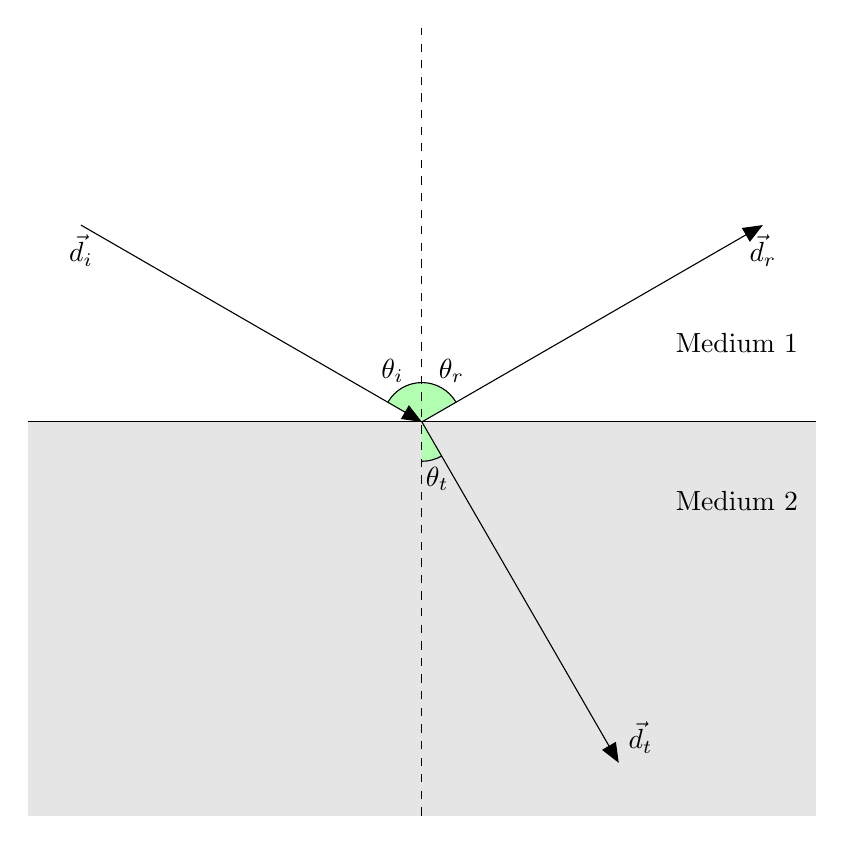
\begin{tikzpicture}
		\newcommand*{\incomingangle}{60}
		\newcommand*{\len}{5cm}
		\tikzset{
			myarrow/.tip={Triangle[length=2.5mm, width=2mm]},
		}
		\coordinate (n1) at (0, \len);
		\coordinate (n2) at (0,-\len);
		\coordinate (r1) at (canvas polar cs:angle=\incomingangle+90,radius=\len);
		\coordinate (r2) at (canvas polar cs:angle=90-\incomingangle,radius=\len);
		\coordinate (r3) at (canvas polar cs:angle={-90 + asin(sin(\incomingangle / 2.00))},radius=\len);
		\coordinate (O) at (0,0);
		\fill[fill=gray!20] (-\len, 0) rectangle (\len,-\len);
		\pic[draw, fill=green!30, angle eccentricity=1.5, "$\theta_i$"] {angle = n1--O--r1};
		\pic[draw, fill=green!30, angle eccentricity=1.5, "$\theta_r$"] {angle = r2--O--n1};
		\pic[draw, fill=green!30, angle eccentricity=1.5, "$\theta_t$"] {angle = n2--O--r3};
		\draw (-\len,0) -- (\len,0);
		\draw[dashed] (n2) -- (n1);
		\draw[-myarrow] (r1) node [below] {$\vec d_i$} -- (O);
		\draw[-myarrow] (O)  -- (r2) node [below] {$\vec d_r$};
		\draw[-myarrow] (O) -- (r3) node [above right] {$\vec d_t$} ;
		\draw (4,1) node {Medium 1}; 
		\draw (4,-1) node {Medium 2}; 

		\undef\incomingangle
		\undef\len
	\end{tikzpicture}
	\caption{Direction of incoming $\vec d_i$, reflected $\vec d_r$ and
	transmitted $\vec d_t$ waves at a boundary between two media according to
	Snell's law. The dotted line is the direction normal to the
	surface. In particular, in the pictured scenario the second medium has an
	index of refraction bigger than the first medium. Therefore we can note
	that the transmitted wave is deflected closer to the normal of the
	surface.}
	\label{fig:refraction}
\end{figure}

We are also interested in how the power of the incident light is distributed
among the reflected and transmitted waves. The power of the reflected light 
for an isotropic medium with conductivity $\sigma = 0$ and permeability equals
to the permeability of free space is related to the incident power by the
Fresnel equations \cite{itu-buildings}:
\begin{gather}\label{eq:fresnel}
	\frac{P_{t\parallel}}{P_{i\parallel}} = \left|\frac{n_2\cos(\theta_i) - n_1 \cos(\theta_t)}{n_2\cos(\theta_i) + n_1 \cos(\theta_t)}\right|^2 \\
	\frac{P_{t\perp}}{P_{i\perp}} = \left|\frac{n_1\cos(\theta_i) - n_2 \cos(\theta_t)}{n_1\cos(\theta_i) + n_2 \cos(\theta_t)}\right|^2
\end{gather}
where $P_{t\parallel}$ ($P_{i\parallel}$) is the power of the transmitted
(incident) wave with polarization parallel to the incident plane and
$P_{t\perp}$ ($P_{i\perp}$) is the power of the transmitted (incident) wave
with polarization perpendicular to the incident plane, $n_1$ is the index of
refraction of the first medium and $n_2$ is the index of refraction of the second 
medium. The index of refraction, apart from the formulation given in
\autoref{iorspeed}, can also be expressed as a function of the relative
permittivity $\epsilon_r$ and relative permeability $\mu_r$ of the medium
\cite{itu-buildings}:
\begin{equation}\label{eq:real-ior}
	n = \sqrt{\epsilon_r}
\end{equation}
Furthermore, for a medium with non zero conductivity $\sigma$, 
we can introduce a complex index of refraction defined as \cite{itu-buildings}:
\begin{equation}\label{eq:complex-ior}
	n = \sqrt{\epsilon_r - j \frac{\sigma}{\epsilon_0 \omega}}
\end{equation}
where $j$ is the imaginary unit, $\sigma$ is conductivity of the material,
$\epsilon_0$ is the permittivity of free space and $\omega$ is the angular
frequency defined as $\omega = 2\pi f$ with $f$ the frequency. It can be noted
that for $\sigma = 0$ the index of refraction reduces to \autoref{eq:real-ior}.

\subsubsection{Total reflection}

\autoref{snell2} does not have a solution for the transmission
angle $\theta_t$ when the index of refraction of the second medium is smaller
than the index of the first and for a large enough incidence angle $\theta_i$.
When those conditions are verified, all the light is reflected and no light is
transmitted. This phenomenon is called total reflection \cite[p.~50]{born}.

The limiting angle of incidence $\overline{\theta}_i$, which when exceeded total
reflection arises, is given by
\begin{gather}
	% \frac{n_1}{n_2}\sin(\overline{\theta}_i) = 1 \\
	\overline{\theta}_i = \arcsin\left(\frac{n_2}{n_1}\right)
\end{gather}

%TODO immagine

\subsubsection{Dependency of material properties on the EM wave frequency}\label{subsub:prop-fit}

\autoref{eq:fresnel} gives a way to compute the reflected and transmitted power
given the angle of incidence and index of refraction. In turns, the index of
refraction depends on the permittivity and conductivity of the material
(\autoref{eq:complex-ior}). However, the same material can behave differently
for different frequencies, thus, in general, permittivity and conductivity
depend on the frequency. Therefore, to derive those electrical properties for a
given frequency, models based on the fitting of real world measures have been
developed. The International Telecommunication Union proposes 
a model based on four parameters $a$, $b$, $c$ and $d$ from which 
permittivity and conductivity are obtained \cite{itu-buildings}:
\begin{gather}
	\epsilon_r = a f_{\text{GHz}} ^ b \\
	\sigma = c f_{\text{GHz}} ^ d 
\end{gather}
where $f_{\text{GHz}}$ is the frequency in giga Hertz. Example of parameters
computed to fit real world measures are shown in
\autoref{table:material-props}, while \autoref{fig:reflectivity} pictures how
the reflectivity is affected by the frequency of the incoming EM wave for the
concrete and wet ground materials.

\begin{table}
	\centering\begin{tabular}{c|cccc|c}
		\toprule
		\textbf{Material class} & $a$ & $b$ & $c$ & $d$ & \textbf{Frequency range (GHz)} \\
		\hline
		Concrete & 5.24 & 0 & 0.0462 & 0.7822 & 1-100 \\
		Wood & 1.99 & 0 & 0.0047 & 1.0718 & 0.001-100 \\
		Metal & 1 & 0 & $10^7$ & 0 & 1-100 \\
		Very dry ground & 3 & 0 & 0.00015 & 2.52 & 1-10 \\
		Medium dry ground & 15 & -0.1 & 0.035 & 1.63 & 1-10 \\
		Wet ground & 30 & -0.4 & 0.15 & 1.30 & 1-10 \\
		\bottomrule
	\end{tabular}
	\caption{Parameters used to compute permittivity and conductivity for
	different materials as recommended by the International Telecommunication
	Union \cite{itu-buildings}. The frequency range corresponds to the
	frequencies used in the measures the parameters are based on.}
	\label{table:material-props}
\end{table}

\begin{figure}
	\centering
	\begin{subfigure}[t]{0.45\textwidth}
		\includegraphics[width=\textwidth]{images/concrete.pdf}
		\caption{Concrete material. The reflectivity does not appear to change
		significantly for 1 and 10 GHz.}
	\end{subfigure}
	\hfill
	\begin{subfigure}[t]{0.45\textwidth}
		\includegraphics[width=\textwidth]{images/wet_ground.pdf}
		\caption{Wet ground material. The reflectivity changes significantly
		for 1 and 10 GHz, especially at low angles of incidence. }
	\end{subfigure}

	% \hfill

	\caption{Reflectivity, given by $\frac{1}{2}
	\left(\frac{P_{t\parallel}}{P_{i\parallel}} +
	\frac{P_{t\perp}}{P_{i\perp}}\right)$, as a function of angle of incidence
	for different frequencies and different materials with the parameters given in \autoref{table:material-props}.}
	\label{fig:reflectivity}
\end{figure}



\subsubsection{Diffusion}

When a surface is rough compared to the wavelength, the reflection is specular
only in a small region. This results, at macroscopic scale, in the wave being
reflected at all angles. This phenomenon is called diffusion or diffuse
scattering \cite[p.~17]{richards2010principles}.

\subsection{Diffraction}

EM waves travel in a straight line in an homogeneous medium and are reflected
or refracted when meeting a boundary between two different medium. However, EM
waves can also interact with object when traveling close to them, resulting in
a bending of the direction of travel towards the geometric shadow region. This
phenomenon is called \emph{diffraction} \cite[p.~140]{richards2010principles}.



\subsection{Propagation of EM waves in the atmosphere}

The atmosphere causes an attenuation of the EM waves that propagate into it.
Two major factor in the attenuation are absorption and scattering
\cite[p.~121]{richards2010principles}. Absorption is caused by lossy media in
the atmosphere, such as oxygen molecules and raindrops, and converts part of
the energy of the wave into heat. Scattering in the atmosphere causes the EM
wave to be reflected in all directions. The atmospheric attenuation is modeled
to depends on an attenuation coefficient $\alpha$ measured in $\text{m}^{-1}$.
Thus, the attenuation, expressed as the ratio of the attenuated power $P_a$ and the
original power $P_0$, is given by:
\begin{equation}
	\frac{P_a}{P_0} = 10^{\alpha \frac{L}{2}}
\end{equation}
where $L$ is the path length in meters. The attenuation coefficient depends on
atmospheric conditions, such as rain intensity, the frequency of the
EM wave but also temperature and altitude.


\section{GPU Programming and the Vulkan API}\label{sec:vulkan}

Vulkan is a graphics and compute API, designed to provide cross-platform access
to modern GPUs \cite{whatisvulkan}. The Vulkan API is defined by a public
specification \cite{vulkanspec} written by the Khronos Group, a non profit
organization developing royalty-free standards \cite{aboutkhronos}.

In Vulkan, shaders are programs run on the GPU. They can be written in high
level languages such as GLSL or HLSL and compiled to a platform-independent
bytecode format, called SPIR-V. Shaders are used in the context of a
\emph{pipeline}. A pipeline constitutes a configuration for how the shaders are
to be used and can be one of three different kinds:
\begin{itemize}
	\item graphics pipeline: used for 2D or 3D rendering;
	\item compute pipeline: used for general purpose GPU programming (GPGPU);
	\item ray tracing pipeline: used to perform ray tracing. 
\end{itemize}
In this work we are mainly interested in the ray tracing pipeline.

\subsection{The ray tracing pipeline}\label{subsec:raytracing}

The Vulkan ray tracing pipeline, introduced by the extension
\verb!VK_KHR_ray_tracing_pipeline! \cite{vulkanraytracingpipeline}, leverages a
dedicated set of shader stages and commands, independent from both the graphics
and compute pipelines. \autoref{fig:raytracingpipeline}
pictures
the five stages supported by the ray tracing pipeline and the interaction among
them.

\tikzstyle{programmable} = [rectangle, rounded corners, minimum width=3cm, minimum height=1cm,text centered, draw=black, fill=blue!30]
\tikzstyle{fixed} = [rectangle, minimum width=3cm, minimum height=1cm, text centered, draw=black, fill=lightgray!30]
\tikzstyle{arrow} = [->,>=stealth]
\tikzstyle{decision} = [diamond, minimum width=1cm, minimum height=1cm, text centered, draw=black, fill=white]
\begin{figure}\centering
	\begin{tikzpicture}[node distance=2cm]
		\node (raygen) [programmable] {Ray Generation shader};
		\node (astraversal) [fixed, below=of raygen] {Acceleration Structure Traversal};
		\node (is) [programmable, right=of astraversal] {Intersection shader};
		\node (any) [programmable, above=of is, yshift=-1cm] {Any Hit shader};
		\node (maybehit) [decision, below=of astraversal, yshift=1cm] {Hit?};
		\node (miss) [programmable, right=of maybehit] {Miss shader};
		\node (closest) [programmable, left=of maybehit] {Closest Hit shader};
		\draw [arrow] (raygen) -- (astraversal);
		\draw [arrow] (astraversal) -- (maybehit);
		\draw [arrow] (maybehit) -- (closest) node [midway, above] {Yes};
		\draw [arrow] (maybehit) -- (miss) node [midway, above] {No};
		\draw [arrow] (astraversal) -- (is);
		\draw [arrow] (is) -- (any);
		\draw [arrow] (any) -| ($(astraversal.north) + (2cm,0)$);
	\end{tikzpicture}
	\caption{Ray tracing pipeline stages. Stages in blue are fully programmable
	with a shader, while the stage in gray is fixed.}
	\label{fig:raytracingpipeline}
\end{figure}

% Explain the various stages

\subsubsection{Ray generation shader stage}\label{subsubsec:raygen}

The ray generation shader is the starting point of the pipeline. A three
dimensional grid of shader invocations is launched with the command
\verb!vkCmdTraceRaysKHR!. A ray is an half-line expressed by the parametric
equation:
\begin{equation}\label{eq:ray}
	r(t) = \vec{o} + t \vec{d}
\end{equation}
where $\vec{o}$ is the origin of the ray, $\vec{d}$ is its direction and $t \ge
0$.

In the shader, each invocation can access to its launch identifier with the
built-in variable \verb!gl_LaunchIDEX! and trace a ray with the
\verb!traceRayEXT! function, passing its origin and direction as defined in
\autoref{eq:ray}, together with a minimum ($t_{min}$) and
maximum ($t_{max})$ value of the parameter, defining an interval in which to
search for intersection with the geometries.

Each ray is associated with a
\emph{payload}, an arbitrary, application-defined data structure which can be
read and written from the various stages of the pipeline.


\subsubsection{Acceleration structure traversal}

An acceleration structure is an implementation-dependant and opaque data
structure used to represent geometric objects and efficiently find which, if
any, primitive is intersected by the traced ray. An acceleration structure can 
either be a bottom level acceleration structure (BLAS), in which case it 
can either store an array of geometries consisting of triangles or axis aligned
bounding boxes, or can be a top level acceleration structure (TLAS), which 
contains an array of BLAS.
During the traversal, an intersection with triangles for parameters in the range
$(t_{min}, t_{max})$ causes invocation of the any hit shader, while an
intersection with an axis aligned bounding box (AABB) causes first invocation
of the intersection shader and possibly then of the any hit shader.


\subsubsection{Intersection shader stage}\label{subsub:intersectionshader}

Intersection shader are used to implement intersections with user-defined
primitives, such as surfaces defined by an equation instead of triangles. When
an intersection with the corresponding AABB is found, this shader is called and
tests whether the primitive is intersected by the ray. If the intersection has
occurred, it uses the \verb!reportIntersectionEXT! function and the
intersection is reported to the any hit shader. Intersection shaders cannot
read or modify the ray payload.


\subsubsection{Any hit shader stage}

An any hit shader is an optional shader whose goal is to confirm or ignore a
reported intersection with an object. This stage can also modify the ray
payload or terminate the tracing of the ray early. A possible use for this
shader is to have partially transparent surface, where the transparency is
defined by a texture.


\subsubsection{Closest hit shader stage}\label{subsubsec:closesthitshader}

When all the intersection of a ray has been determined, the closest hit shader is
called for the closest one (i.e.~the one with minimum value of the parameter
$t$), if it exists. In this stage the payload can be modified and it is also
possible to recursively trace new rays with \verb!traceRayEXT!.
Shaders in this stage have access to useful built-in variables:
\begin{itemize}
	\item \verb!gl_InstanceID!, containing the index of the BLAS instance the
		intersection happened with;
	\item \verb!gl_GeometryIndexID!, containing the index of the geometry in the
		BLAS;
	\item \verb!gl_PrimitiveID!, the index of the intersected triangle.
\end{itemize}
Together, those three variable allows to unambiguously identify with which triangle
the intersection happened.


\subsubsection{Miss shader stage}

When no intersection is detected, the miss shader. In this shader the ray
payload can be written to.


\subsubsection{Shader binding table}\label{subsec:sbt}

A ray tracing pipeline may contain more than one shader of the same kind, for
example multiples closest hit shaders. In that case, the acceleration structure
traversal needs additional information in order to choose which shader to call.
This information is available in the form of the \emph{shader binding table}
\cite[p.~192]{gemsII}.
The shader binding table stores handles which refer to the shader records, possibly
together with embedded parameters. There are three
different kinds of shader records: the ray generation record, which contains
just the ray generation shader, the miss record, containing the miss shader,
and the hit group record, which can contain the closest hit, any hit and
intersection shaders. The mechanism used for the selection of a shader record
depends on the shader record type and it is explained in details in the
following paragraphs.

For the hit group record, the selected group is given by the hit group record
index $H_\text{index}$:
\begin{equation}
	H_\text{index} = I_\text{offset} + R_\text{offset} +
	R_\text{stride} \cdot G_\text{id}
\end{equation}
where $I_\text{offset}$ is specified for each BLAS when building a TLAS with
the \texttt{instanceShaderBindingTableRecordOffset} field in the structure
\texttt{VkAccelerationStructureInstanceKHR}, $R_\text{offset}$ and $R_\text{stride}$
are both passed as argument to the function \texttt{traceRayEXT}, $G_\text{id}$
is the index of the geometry in BLAS. This allows to control the used shader group
both on a per-object basis, with $I_\text{offset}$ and $G_\text{id}$, and on a
per-ray basis, with $R_\text{offset}$ and $R_\text{stride}$.


The miss group shader to use is simply specified by the argument
\texttt{missIndex} in \texttt{traceRayEXT}.

\subsection{Comparison between Vulkan and other GPU programming API and platform}

OpenGL is an other graphic API with wide support across hardware vendors and
operating systems, whose standard is maintained by the Khronos Group.
Furthermore, since version 4.3, it supports GPGPU with compute shaders
\cite{opengl43}. OpenGL, however, does not support hardware-accelerated ray
tracing \cite{unterguggenberger2023vulkan}, rendering it unsuitable for this
work.

DirectX is a collection of API designed by Microsoft and available on the
Microsoft platforms. Since version 12, DirectX includes support for hardware
accelerated ray tracing \cite{gemsdx}. Using DirectX, however, limits
application support to the Microsoft platforms such as the Windows operating
system.

OptiX \cite{optix} is a proprietary framework for ray tracing developed by
NVIDIA. It supports Windows, Linux and OSX but only NVIDIA GPUs of the Maxwell
generation or newer.

\autoref{gpuapi} 
summarize the differences relevant for this work of the discussed GPU APIs.

\begin{table}
	\begin{center}
		\begin{tabular}{|c|c|c|c|c|}
			\hline
			& \thead{OS agnostic} & \thead{Hardware vendor \\ agnostic} & \thead{GPGPU programming \\ support} & \thead{Support for hardware \\ accelerated ray-tracing} \\
			\hline\hline
			% CUDA & \textbullet & & \textbullet & \\
			OpenGL & \textbullet & \textbullet & \textbullet & \\
			\hline
			DirectX 12 & & \textbullet & \textbullet & \textbullet \\
			\hline
			OptiX & \textbullet & & \textbullet & \textbullet \\
			\hline
			Vulkan & \textbullet & \textbullet & \textbullet & \textbullet \\
			\hline
		\end{tabular}
	\end{center}
	\caption{Summary of GPU programming APIs support for different operating
	systems, hardware vendors and hardware ray-tracing acceleration.}
	\label{gpuapi}
\end{table}


\section{Hardware accelerated ray tracing}\label{sec:hw-rt}

In September 2018, NVIDIA introduced in theirs GPU, with the Turing
architecture, the \emph{RT Cores}. RT Cores are dedicated to the acceleration
of the traversal of bounding volume hierarchies (BVH) and the testing of
ray/triangle intersection \cite{turing-whitepaper}. RT Cores therefore allow to
offload the Streaming Multiprocessor, which meanwhile can carry out other
computations. Sanzharov et al.~\cite{rtxexamination} show that ray tracing
implementation using the new RT Cores are from 2 to 5 times faster with respect
to existing software based ray tracers. They observe that the higher speedups
happen with rays with random directions, which require random memory access to
traverse the BVH. Therefore they speculate that the new hardware is capable of
reordering memory accesses caused by BVH traversal.

AMD as well introduced in their RDNA2 architecture ray accelerators.
RDNA2 ships with one ray accelerator with each of their Compute Units (CUs) \cite{rdna2}.
Those ray accelerators execute two new instructions, dedicated to the intersection test
of bounding volume hierarchies and triangles with rays \cite{rdna2}.


\chapter{Level-7 Switch}\label{ch:method}

In this chapter, we present our Layer-7 switch using AF\_XDP technology and its application to a simulated maritime operational technology system.
In particular, we will highlight the differences between a traditional Layer-2/Layer-3 switch and our implementation, with a focus on its smart-filtered data flow.
The following sections describe in great detail the analysis steps leading to the final project architecture.

\section{From L2 to L7}
When we talk about a "layer" in switch terminology, we are referring to the Open System Interconnection (OSI) layer the switch operates on.
Today's implementations, applied to maritime OC systems, work on the the Data Link layer (L2) operating eventually on the Network Layer (L3).
The lower one being responsible for MAC-Address based forwarding of data frames.

Traditionally network device interfaces (NICs), each one with a unique MAC address, are connected to the switch via physical Ethernet ports or fiber optic ports depending on speed requirements.
When a NIC sends data to the switch its MAC address is inserted inside a very simple data structure, called the MAC address table, which contains basic routing information.
If the table contains the packet's destination address, the packet is routed to the associated port otherwise it is sent to all ports except the sender's, creating a packet "flood".

Requiring no routing algorithm, and not needing IP addresses to forward data, Layer 2 switches are very fast, and cost less than routers. However, broadcast traffic is not controlled leading to network congestion while handling high workloads. Lastly, these kind of switch cannot pass data between different VLANs precluding network segmentation.

Faced with the practical and performance limitations of lower-layer switches, there has been a move toward Layer 3 implementations, especially in industrial network topologies.
To ensure flexible application planning a host of Network Layer features are quickly became “must haves”.

Layer 3 packet routing is performed by routers that use IP addresses instead of MAC addresses, making this new paradigm ideal for local area networks. Switches that use this strategy can connect different VLANs, provide more security features, and apply Quality of Service (QoS) controls for maximum efficiency. 

Using an ARP table data structure which shows both MAC and IP addresses, switches will either forward the packet like a Layer 2 switch, or route it according to a routing protocols.

\leavevmode\newline
\begin{tabularx}{\textwidth}{|>{\hsize=0.5\hsize}X|>{\hsize=0.5\hsize}X|}
  \hline
  \multicolumn{2}{|c|}{\textbf{L2/L3 Features}} \\ \hline
  L2 & L3 \\ \hline
  Sends data “frames” to destination MAC address & Routes data “packets” based on MAC or IP address\\ \hline
  OSI Layer 2 (Data Link Layer) & OSI Layer 3 (Network Layer)\\ \hline
  Cannot connect different VLANs & Able to connect different VLANs\\ \hline
  One broadcast domain & Multiple broadcast domains \\ \hline
  Communicates with local network & Can connect to outside (multiple) networks\\ \hline
\end{tabularx}
\leavevmode\newline \\



\chapter{Implementation}\label{ch:implementation}

In this chapter, the focus will be on the implementation choices made for the realization of the Layer 7 switch.
We will analyze the programming language, algorithms, data structures, and libraries used to optimize efficiency, modularity, and interaction with the underlying technologies discussed previously. 

\section{Enviroment setup}
From the beginning, our switch was designed to be placed inside a maritime operational technology system, such as a ship, to monitor its internal network.

Since it was not possible to test the software against a physical infrastructure, the creation of a virtual twin seemed the most reasonable choice. In addition, the first step toward legacy compatibility was the ability to run the software on commodity hardware such as a personal computer, which has very limited resources compared to industrial system components.

\subsection{Linux Network-Namespaces}
Linux network-namespaces are a powerful feature that allows users to create isolated network environments within a single host, making them a valuable option for emulation, testing, and development, as they provide a controlled environment in which network configurations can be set up without affecting the host system or other network environments.
Simulations such as the one we focused have core logic that can span multiple, separate environments, making it necessary to be network namespace, or container, aware. By creating a completely new network stack within a namespace for each system component, the containers can completely isolate their network environments from each other, perfectly simulating an industrial environment where each device is a separate entity with its own life cycle.

Taking advantage of the containerization capabilities of the technology, we automated the creation of a simple but complete OT system with a single Makefile.\\

\begin{lstlisting}[language=make]
CONTAINERS := 1 2 3 4 5 6 7 8

.PHONY: test-container-%
test-container-%:
	$(eval I := $(subst test-container-,,$@))
	sudo ip netns add test$(I)
	sudo ip netns exec test$(I) ip link set dev lo up
	sudo ip netns exec test$(I) ip link add eth0 type veth peer name test$(I)
	sudo ip netns exec test$(I) ip link set dev test$(I) netns 1
	sudo ip netns exec test$(I) ip link set dev eth0 address 54:00:00:00:00:$(I)0
	sudo ip netns exec test$(I) ip addr add 10.42.0.$(I)0/24 dev eth0
	sudo ip netns exec test$(I) ip link set dev eth0 up
	sudo ip netns exec test$(I) ip neigh add 10.42.0.$(I) lladdr 54:00:00:00:00:0$(I) nud permanent dev eth0
	sudo ip link set dev test$(I) up
	sudo ip link set dev test$(I) address 54:00:00:00:00:0$(I)
	sudo ip addr add 10.42.0.$(I)/32 dev test$(I) noprefixroute
	sudo ip route add to 10.42.0.$(I)0/32 dev test$(I) src 10.42.0.$(I)
	sudo ethtool -K test$(I) tx off
	sudo ip netns exec test$(I) ethtool -K eth0 tx off

.PHONY: test-net
test-net: $(foreach container,$(CONTAINERS),test-container-$(container) )
\end{lstlisting}

This file alone is enough to configure a completely reliable simulation of a possible infrastructure we might find on a ship.Eight network namespaces representing different physical components are created, and for each one a virtual Ethernet interface is also set up and paired with the loopback interface of the host machine that was previously brought up. As mentioned earlier, in keeping with namespace theory, each container is considered a separate device with its own MAC address, IP address, and network stack.
To be consistent with packet routing and to have a simulation as close to a real context as possible, transmit checksum offloading has also been disabled to avoid unexpected behavior due to the abstraction layers of network virtualization.

\begin{figure}[H]
	\centering
    \includegraphics[scale=0.4]{thesis/images/network_namespaces.png}
	\caption{Visualization of Linux Network Namespaces}
    \label{fig:network_namespaces}
\end{figure}

The only drawback of using network namespaces could be identified in the use abstraction layers of some kind that may give unrealistic results with slower or faster performance compared to the physical counterpart. But for the sake of research and study on the applicability of new networking strategies to legacy systems, our concerns for this part are mainly focused on the reproducibility of the network topology.

\section{The Rust Programming Language}
\section{Project Layout}
\section{Algorithmic choices and Crates}
\section{Implementation's highlights}





%\chapter{Results}
\label{ch:results}

In this chapter, an analysis is conducted of the results obtained from the execution of multiple tests on the software under investigation. Since tests over the implementation's correctness are trivial by design the focus is on network speed. The results are then compared with the performance of OT systems traditional networking techniques. Furthermore, an assessment is made of the advantages and disadvantages of the L7 switch. 

\section{Linux baseline }





%\chapter{Related Work}
\label{ch:related}

% This chapter is dedicated to the work that has been done by others in the field of your thesis.
% Don't write a mere list of papers with a summary of each. Instead, the goal is to give a picture
% of how your work is situated in the context of the work of others. In this case, you should
% think your skeptical reader is asking ``hasn't this been solved already?''.
%
% There will be two main kinds of work that you will need to discuss: work that is similar
% to yours, and work that is complementary to yours.
%
% Similar work will try to solve the same problem you are addressing, or a similar one.
% Here, you should focus on the differences: for example, you may write something along the
% lines of ``\textcite{DBLP:journals/x/Turing50} provides a naïve definition of
% `intelligent machine', which has this and that limitation. Our work is similar to
% \citeauthor{DBLP:journals/x/Turing50}, but we address these problems by doing this and
% that''.\footnote{Don't be arrogant! I called Turing's work naïve as a joke.
% For sure your work will have limitations that other work
% may not have, and you should be honest about them.}
%
% Complementary work does not try to solve the same problem you are addressing, but it is
% important to get a full picture of your contribution. For example, if you are
% \emph{not} attempting to solve a particular problem (it is ``out of scope'' for your work),
% but the solution to that problem is necessary for your work to be useful, you should explain
% that here.
%
% While doing your review of related work, \href{https://scholar.google.com}{Google Scholar}
% is probably the easiest search engine for academic papers. You can be mindful of some
% bibliometric tricks to understand which papers are likely to be most influential in the field.
% You can see on Scholar the number of citations of a paper;
% \href{https://portal.core.edu.au/conf-ranks/}{CORE} and
% \href{https://www.scimagojr.com}{Scimago} provide rankings of conferences and journals
% respectively. Non-peer-reviewed articles like those published only on
% \href{https://arxiv.org}{arXiv} may, of course, be important, but you should be more careful
% and skeptical about them.
%
% Wikipedia is a great source of information, but you shouldn't consider it as reliable.
% Wikipedia articles should always provide the sources of the information they contain; you
% should check it yourself, judge its reliability, and cite the original source.
%
% If a paper is very important with respect to your own piece of work, have a look at papers
% that cited it, to see if there are more recent works that are relevant to your thesis.
%
% Here are a few tricks about how to cite other pieces of work:
% \begin{itemize}
%   \item If a paper is available in a peer-reviewed venue (journal or conference), cite that
%   version rather than the non-reviewed one. Sometimes papers are published in two similar
%   versions: one in a conference and an extended one in a journal. In that case, cite the
%   journal.
%   \item Use citations such as ``The Hamiltonian cycle problem is
%   NP-complete~\cite{DBLP:conf/coco/Karp72}'' or ``\textcite{DBLP:conf/coco/Karp72} showed
%   that the Hamiltonian cycle problem is NP-complete''. Don't write
%   ``\cite{DBLP:conf/coco/Karp72} showed that the Hamiltonian cycle problem is NP-complete''.
%   \item \href{https://dblp.org}{DBLP} is a good source of quality Bibtex records for papers
%   you may want to cite.
%   \item You are likely to cite a lot of work that is published on the Web.
%   \href{https://bibtex.eu/faq/how-can-i-use-bibtex-to-cite-a-website/}{Here} is some
%   documentation about how to cite a website.
% \end{itemize}

\section{EM waves propagation modeling and simulation}

Many different techniques for the modeling of EM waves, in particular in the
radio frequency range, have been researched and developed, each with different
degrees of fidelity, flexibility and performances. The most accurate models,
such as the method of moments, solve numerically the integrals and the
differential equations that govern the interaction between EM waves and matter.
While those methods achieve great accuracy, their computational requirements,
both in terms of memory and time, are prohibitive when the modeled
environment is large compared to the wavelength of the wave \cite{Yun}.
Therefore, in practice, the use of such models is limited to small scenes such
as the computation of the radiation pattern of an antenna \cite{matlabpattern},
or the computation of the radar cross section of a single target \cite[Chapter
14]{radarhandbook}.

An alternative method which does not suffer from the same proibitive
performances is the ray tracing method. The ray tracing method works under the
assumption that the wave length is small compared to the size of the targets.
Under this assumption EM waves behave similar to visible light, obeying the
laws of reflection, refraction and diffraction \cite{Yun}. This method
is called shooting and bouncing ray (SBR) because in order to determine the paths
from the transmitting antenna to the receiving one, rays are shot from the
transmitting antenna and then, after possibly bounce on the objects
constituting the environment, checked whether they are received by the receiving
antenna. The SBR method is explained in detail in the following section.

\section{The shooting and bouncing ray (SBR) method}\label{sec:sbr}

The SBR method computes the possible paths from a
transmitting antenna to a receiving one, either propagating directly (line of
sight propagation), or propagating by first interacting with one or more
objects in the environment by means of reflection, transmission and
diffraction. The SBR method has been used first in the computing of 
the radar cross section of a cavity \cite{Ling}, and then it has been
adopted for the prediction of radio wave propagation in urban environment
\cite{Ikegami} \cite{Seidel} and radar simulations \cite{Hirsenkorn}
\cite{scalabledigitaltwins} \cite{mimo}.

In the shooting and bouncing ray method, rays are traced from the transmitting
antenna into the simulated environment, which consists of 3D objects, typically
modeled as a collection of triangle meshes. Objects in the environment are
associated with electrical properties that define how the rays interact with it
when and if they intersect the object. The receiving antennas are modeled as
spheres, which, when reached by a ray, store the information associated to it,
i.e.~ the energy and it carries, its frequency and the distance it traveled.
The information of associated with all the received rays is the output of the
simulation. Therefore three distinct steps can be identified: ray launching,
ray tracing and finally ray reception.

\subsection{Ray launching}

In the shooting and bouncing ray method a transmitting antenna is modeled as a
point source emitting a spherical wavefront in all directions. Therefore, the
rays used in the SBR model are emitted from the same origin, the location of
the transmitting antenna, uniformly distributed over all directions so that to
each ray can be associated roughly the same region of the spherical wavefront.
Rays can therefore be seen as cones or tubes, to which some energy is
associated. Dividing the spherical wavefront uniformly can be achieved by
subdividing the faces of an icosahedron \cite{Yun} or by using the Fibonacci
lattice method \cite{Hirsenkorn}. Each ray cone or tube is in charge of
simulating the propagation of the region of wavefront associated with it.
Furthermore, the further the ray travels, the bigger the cross section of the
tube or cone becomes. This accounts for the spreading factor which reduces the
density of the energy by the square of the distance \cite{Iskander}.

\subsection{Ray tracing}

In the SBR method, before we can know whether a ray is received by an antenna
we need to simulate its propagation. To this end, each of the generated ray is
tested for intersections against the simulated objects. A na\"ive approach
which tests every object in the simulated environment results in this step of
the simulation to become, when a high number of object is required, very
expensive. Thus, techniques to efficiently find if a ray intersect an object
have been employed, such as the bounding volume hierarchy. When an intersection
with an object is found, depending on its electrical properties, the ray is
either reflected, transmitted, diffused or diffracted.

\subsection{Ray reception}

In the ray tracing method the receiving antenna is, like the transmitting one,
modeled as point. Therefore, to establish whether a ray is received, it is
necessary to test if the receiving point resides inside the ray cone or tube.
This is done by placing a reception sphere at the location of the receiving
antenna, whose radius depends on both the angular separation between rays and
the distance the ray has traveled so far \cite{Yun}. The varying size of the
reception sphere ensures that exactly one ray from a given path is received. In
particular, a reception sphere that is too big would receive duplicate rays for
the same path, erroneously receiving more power than it should. On the other
hand, a too small receiving sphere would fail to account for all the path.


\section{SBR in radar simulation}

The problem of simulating a radar is fundamentally similar to the one of
predicting path losses and delays between antennas: there are transmitting and
receiving antennas, which in the case of monostatic radar can be the same, and
environment in which the EM waves propagates. For this reason the SBR method,
originally developed for the simulation of propagation of EM waves, has found
application for radar simulations.

Hirsenkorn et al.~\cite{Hirsenkorn} apply the shooting and bouncing ray method
for the simulation of frequency-modulated continuous-wave radars. For the
generation of rays with non overlapping and roughly equal tubes they leverage
the Fibonacci spiral, assigning to each ray a tube with an hexagonal cross
section. For the reception of the ray, in order to simplify the computation,
they consider, instead of the hexagon-shaped tube, a cone with a cross section
with area equal to the area of the hexagon. Using the NVIDIA OptiX framework,
they mange to trace 50000 initial rays at frame rate of 10 Hz in a scene with
326831 triangles. Finally, they validate the results from the simulation
against real world measures in a motorway scene, showing a good agreement
between simulation and measures.

Schüßler et al.~\cite{mimo} present a simulator for \emph{multiple-input
multiple-output} (MIMO) radars. They use a variant of the SBR method in which
rays, instead of representing the propagation of a region of the spherical
wavefront, are used to approximate the power flux in an area. In this way,
probabilistic materials are possible, allowing for the simulation of diffusing
materials. The probabilistic approach also requires to change the reception of
rays: the reception sphere is now fixed in radius. The interpretation of this
is that, since the number of rays in an area approximates the power flux
density there, with a fixed size reception sphere we are estimating the power
density around the receiving antenna. A downside of the fixed radius sphere is
that the choice of the radius can affect the quality of the simulation result,
as Schüßler et al.~show. Furthermore, Schüßler et al.~use OptiX to leverage the
parallelism of NVIDIA GPUs and are able to trace 1 billion rays in 4 minutes
and 44 seconds.

Buddendick et al.~\cite{Buddendick} propose the use of \emph{scattering
centers} to speed up SBR methods. With scattering centers, a complex object is
approximated by a finite number of points to which it is associated a lookup
table containing its pre-computed scattering properties. More precisely, this
table is a four dimensional matrix storing for each discretized incoming
direction and for each discretized outgoing direction, the bistatic radar cross
section of the part of the object associated with the scattering center.


% \begin{itemize}
% 	\item \cite{Fernando} does not have doppler.
% \end{itemize}


\section{Other methods for radar simulation}

A different approach from SBR is the use of depth images to simulate radars. A
depth image is an image, commonly used in computer graphics, containing at each
pixel the distance, along the line of sight, of the first visible surface. With
the distance, the power received by the object at each pixel is computed and
then, accounting for the material properties and surface normal the reflection
is calculated. The main advantage of this technique with respect to SBR is
performances, as generating a depth buffer is a fast operation. However,
approaches based on the depth buffer assume a single reflection of the EM wave,
i.e.~the transmitted wave hits the object and is reflected back at the location
of the transmitted itself. This assumption renders impossible the simulation of
bistatic radars, for which the location of the receiving antenna differs from
the one of the transmitting antenna, and the simulation of multipath
propagation, i.e.~multiple reflections with objects before reception, which can
give rise to interferences or false echoes.

Schöffmann et al.~\cite{vira} present a simulator for frequency-modulated
continuous-wave radars, based on the generation of depth images and is
implemented in the proprietary game engine Unity. Schöffmann et al.~compute the
contribute to the received power from each pixel given the distance of the
object as stored in depth image. 

Vasstein et al.~\cite{vasstein2020autoferry} leverage the Unity game engine to
simulate infrared sensors, radars and lidars. Similarly to Sch\"offman et al.,
the radar simulation is again based on the use of depth buffers and therefore
does not account for multipath propagation. The authors show that the simulated
radar image looks more detailed than it should be when compared to real world
data.

Ciarambino et al.~\cite{ciarambino2021game} use the Unreal Engine with
Microsoft AirSim to simulate millimiter wave radars in flight settings. They
use the information available from a depth buffer and normal maps to compute
the power return using a radar equation that accounts for atmospheric loss.
They approximate the radar cross section with the Phong illumination model.

Leite et al.~\cite{leite2023low} use the Unity game engine to simulate radars
in maritime scenario. They leverage a depth and normal buffers to generate the
radar returns with low fidelity but real time performances. In particular,
they consider the signal reflected back to the radar when the surface normal
is close to being perpendicular to the line of sight. They also account
for false echoes by duplicating the echoes at a multiple of the distance.

\section{Commercial solutions}

MATLAB implements the shooting and bouncing ray method in the Antenna Toolbox \cite{antennatoolbox} 
to compute the propagation paths and their losses between two antennas. While this solution can 
predict the signal strengths and propagation delays, it suffers from limitations that render 
it inadeguate with respect to the goal defined \autoref{sec:goals}. Indeed, the 
simulation happens in static static environment, with no possibility of modeling
moving objects and doppler shifts. Furthermore, performances are incompatible with 
real-time constraint (see \autoref{sec:benchmark} for a comparison with our work). Also, 
the Antenna Toolbox does not support the use of a single antenna for both transmission and
reception, as in the configuration of a monostatic radar.


%% vim: ft=tex
\chapter{Conclusion and Future Work}
\label{ch:conclusion}
 
In this study, we presented a simulation of a Layer 7 Switch that was based on the AF\_XDP technology applied to a maritime OT system. This simulation was successful in achieving the initial objectives that were established. In fact, our software is entirely agnostic to the underlying software and hardware. The only software dependency of our software is the Linux kernel, and it does not require additional physical components.
Additionally, our implementation can be seamlessly integrated into existing systems without altering standard communication protocols or introducing new ones preserving the transparency feature. Finally, it does not alter the normal communication flow and is able to handle, filter, and process NMEA traffic without adding any performance overhead, as evidenced by the obtained results.

It is possible that enhancements may be implemented, including software refinements. The main one being the implementation of a crate/library that is independent from the C libbpf library. This would ensure complete system fault-proofing, a characteristic facilitated by the Rust programming language features. Prior to contemplating additional any other enhancement excluding the aforementioned, it is essential that the software undergoes testing on real industrial systems. This evaluation may identify other software features that could prove beneficial.


%\printbibliography

\end{document}

